\documentclass{tufte-book}
\usepackage[utf8]{inputenc}
\usepackage{cite}
\usepackage{url}
\usepackage{booktabs}
\usepackage{hyperref}
\hypersetup{
colorlinks=true,
linkcolor=blue,
filecolor=red,
urlcolor=blue,
}

\usepackage{graphicx}
\usepackage{tikz}
\usetikzlibrary{decorations.pathmorphing}
\tikzset{snake it/.style={decorate, decoration=snake}}
\usetikzlibrary{decorations.markings}
\tikzset{middlearrow/.style={ decoration={markings, mark= at position 0.575 with {\arrow{#1}}, }, postaction={decorate} } }
\usepackage{amsmath,amssymb}
\usepackage{physics}
\usepackage{mathtools}
\usepackage{marginfix}

\setcounter{secnumdepth}{4}
\setcounter{tocdepth}{1}

\title{Group Theory in Physics}
\author{Meng Sun}

\newcommand{\bp}{\mathbf{p}}
\newcommand{\bq}{\mathbf{q}}
\newcommand{\bk}{\mathbf{k}}
\newcommand{\br}{\mathbf{r}}
\newcommand{\bL}{\mathbf{L}}


\begin{document}
\maketitle
\tableofcontents

\chapter{BASIC GROUP THEORY}

\section{Basic Definitions and Simple Example}
\textbf{Definition 1.1, Group} A set $\{G: a, b, c\dots\}$ is sai to form a group if there is an operaton called \textit{group multiplication}, which associates any given pair of elements $a, b \in G$ with a well-defined product $a \cdot b$ which is also an element of $G$, such that the following  condition are satisfied:
\begin{itemize}
  \item The operation $\cdot$ is associative, $a \cdot \left(b \cdot c\right) = \left(a\cdot b \right) \cdot c$for all $a, b, c \in G$;
  \item Among the elements of $G$, there is an element $e$, called the identity;
  \item For each $a \in G$, there is an inverse element, $a \cdot a^{-1}=e$.
\end{itemize}

\textrm{Example 1}: The $C_{2}$ group.
There are two group elements with the multiplication table in Tab.~\ref{tab:1-1}
\begin{table}
  \centering
  \begin{tabular}{c c}
    \hline
    e & a \\
    a & e \\
    \hline
  \end{tabular}
  \caption{Group Multiplication Table of $C_{2}$}
  \label{tab:1-1}
\end{table}
In physics, the spatial inversion transformation and identity form such a group.

\textit{Example 3}: There is one and only one three-element group called $C_{3}$ and the multiplication table is Tab.~\ref{tab:1-2}.
\begin{table}
  \centering
  \begin{tabular}{c c c}
    \hline \\
    e & a & b \\
    a & b & e \\
    b & e & a \\
    \hline
  \end{tabular}
  \caption{Group Multiplication Table of $C_3$}
  \label{tab:1-2}
\end{table}
Since $ab=e$ we conclude $b=a^{-1}$, we can denote the three elements by $\{e, a, a^{-1}\}$ with the requirement $a^{3}=e$.
Concrete examples of the the group $C_{3}$ are: the numbers $\left( 1, e^{i2\pi/3}, e^{-i2\pi/3}\right)$ with the usual rules of multiplication; the symmetry operations of the equilater trangle in the plane.

All these groups mentioned are examples of \textit{cyclic} group $C_{n}$ which have the general structure $\{e, a, a^{2}, \dots, a^{n-1}; a^{n}=e\}$ where $n$ can be any positive integer.

\textbf{Definition 1.2, Abelian group} An \textit{abelian group} $G$ is none for which the group multiplication is commutative.

\textbf{Definition 1.3, Order} The \textit{order} of a group is the number of elements of the group.

The cyclic groups $C_{n}$ described abover are all abelian.
Most interesting groups are not abelian.

\textrm{Example 4}: The simplist non-cyclic group is of order $4$.
It is usually called the \textit{dihedral group} denoted by $D_{2}$ with the multiplication table Tab.~\ref{tab:1-3}
\begin{table}
  \centering
  \begin{tabular}{c c c c}
    \hline
    e & a & b & c \\
    a & e & c & b \\
    b & c & e & a \\
    c & b & a & e \\
    \hline
  \end{tabular}
  \caption{Group Multiplication Table of $D_2$}
  \label{tab:1-3}
\end{table}

A visualize of this abelian group is by its association to a geometrical symmetry by considering the configuration of
Fig.~\ref{fig:1-1}.
\begin{figure}[h]
  \centering
  \begin{tikzpicture}
    \draw (0,0) -- (0,2) -- (4,2) -- (4,0) -- (0,0);
    \draw (0,1) -- (4,1);
    \draw (2,0) -- (2,2);
    \node [left] at (0,1) {$4$};
    \node [right] at (4,1) {$2$};
    \node [below] at (2,0) {$3$};
    \node [above] at (2,2) {$1$};
  \end{tikzpicture}
  \caption{A configuration with $D_2$ symmetry.}
  \label{fig:1-1}
\end{figure}
Applying the following tansformations on this figure: (i) leaving the figure unchanged; (ii) reflection about the vertical axis $(1,3)$; (iii) reflection about the horizontal axis $(2,4)$; and (iv) rotation of the figure in the plane around the center by $\pi$.
It is straightforward to check that the multiplication thable obtained through these geomentric constructions reproduces Tab.~\ref{tab:1-3}.

\section{Further Examples, Subgroups}
The smallest \textit{non-abelian group} is of order $6$.
It can be generated from the symmetry transformations of the geometric configuration of Fig.~\ref{fig:1-2}.
\begin{figure}[b]
  \centering
  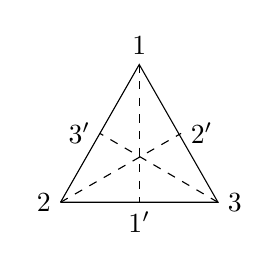
\begin{tikzpicture}
    \draw (0,0) -- (2,0) -- (1, 1.75) -- (0,0);
    \draw [dashed] (0,0) -- (1.531,0.875);
    \draw [dashed] (2,0) -- (0.5,0.875);
    \draw [dashed] (1,1.75) -- (1,0);
    \node [above] at (1,1.75) {$1$};
    \node [right] at (2,0) {$3$};
    \node [left] at (0,0) {$2$};
    \node [below] at (1,0) {$1'$};
    \node [right] at (1.531,0.875) {$2'$};
    \node [left] at (0.5,0.875) {$3'$};
  \end{tikzpicture}
  \caption{A configuration with $D_3$ symmetry}
  \label{fig:1-2}
\end{figure}
The operations are (1) the identity transformation, (ii) reflections about the axes $\left(1,1'\right)$ and so on and (iii) the rotations about the center by angles $\frac{2\pi}{3}$ and $\frac{4\pi}{3}$.
They form the \textit{dihedral group} $D_{3}$.
The reflecvtions interchange two fo the labels, leaving the remaining one unchanged, which we denote the oberation by $\left( 12\right)$.
For rotation counter-clockwise by $\frac{2\pi}{3}$ and $\frac{4\pi}{3}$ we deonte by $\left(321\right)$ and $\left(123\right)$ respectively.
One can see that there is a one-to-one correspondence between these symmetry transformations and the permutations of ther tree label whic form the permutation group $S_{3}$ in next section.
The group multiplication table is shown in Tab.~\ref{tab:1-4}.
\begin{table}
  \centering
  \begin{tabular}{c c c c c c}
    \hline \\
    $e$ & $\left(12\right)$ & $\left(23\right)$ & $\left(31\right)$ & $\left(123\right)$ & $\left(321\right)$ \\
    $\left(12\right)$ & $e$ & $\left(123\right)$ & $\left(321\right)$ & $\left(23\right)$ & $\left(31\right)$ \\
    $\left(23\right)$ & $\left(321\right)$ & $e$ & $\left(123\right)$ & $\left(23\right)$ & $\left(12\right)$ \\
    $\left(31\right)$ & $\left(123\right)$ & $\left(321\right)$ & $e$ & $\left(12\right)$ & $\left(23\right)$ \\
    $\left(123\right)$ & $\left(31\right)$ & $\left(12\right)$ & $\left(23\right)$ & $\left(321\right)$ & $e$ \\
    $\left(321\right)$ & $\left(23\right)$ & $\left(31\right)$ & $\left(12\right)$ & $e$ & $\left(123\right)$ \\
    \hline
  \end{tabular}
  \caption{Group Multiplication Table of $D_3$ or $S_3$}
  \label{tab:1-4}
\end{table}

\textbf{Definition 1.4, Subgroup} A subset $H$ of a group $G$ which forms a group under the same multiplication law as $G$ is said to form a \textit{subgroup} of $G$.

\textrm{Example 1} The group $S_{3}$ has four distinct subgroups consisting of the elements $\{e, \left(12\right)\}, \{e, \left(23\right)\}, \{e, \left(31\right)\}$ and $\{e, \left(123\right), \left(321\right)\}$ respectively.
The first three subgroups are identcal to the $C_{2}$ group.
The last one has the structure of $C_{3}$.
This can be seen by refering to the geometrical transformations in Fig.~\ref{fig:1-2}.

In many applications, the group elements carry labels which are continuous parameters.
These are \textit{continuous groups}.
Group of rotations in Euclidean spaces, and groups of continuous translations areprominent examples.
For later useage, we refere to the groups of ratiotions in space as $R\left(n\right)$ and the comined groups of rotations and translations in the same space as $E_{n}$.
The latter two are examples of \textit{Euclidean groups}.

Any set of invertible $n\times n$ matrices, which includes the unit matrix and which is closed under matrix multiplication, forms a \textit{matrix group}.
Important examples are:
\begin{itemize}
  \item the general \textit{linear group} $GL \left(n\right)$ consisting of all invertible $n\times n$ matrices;
  \item the \textit{unitary group} $U \left(n\right)$ consiting of unitary matrices, $U U^{\dagger} =1$;
  \item the \textit{special unitary group} $SU\left(n\right)$ consisting of unitary matrices with \textit{unit determinant} $\det{U}=1$;
  \item the \textit{orthogonal group} $O \left(n\right)$ consisting of real orthogonal matrics $OO^{T} = 1$.
\end{itemize}

These are examples of classical groups which occupy a central placew in group representation theory and have many applications in various branches of mathematics and physics.
Clearly, $SU\left(n\right)$ and $O\left(n\right)$ are subgroups of $U\left(n\right)$ which, in turn, is a subgroup of $GL\left(n\right)$.

\section{The Rearrangement Lemma and the Symmetric Group}
\textbf{Rearrangement Lemma:} If $p, b, c \in G$ and $pb = pc$ then $b=c$.

This result means: if $b$ and $c$ are distinct elements of $G$, then $pb$ and $pc$ are also distinct.
Therefore, if all the elements of $G$ are arranged in a sequencse and are multiplied on the left (right) by a given element $p$, the resulting squence is just a rearrangement of the original one.

Let us consider a finite group of order $n$, which is $\{g_{i}; i = 1,\dots, n\}$.
Multiply by $h\in G$ which is $g_{h_{i}} = hg_{i}$, then these $h_{i}$ are just the rearrangement of the label $i = 1, \dots, n$ and they must be distinct with each other due to the rearrangement lemma.

We introduce the \textit{group of permutations}.
An arbitrar permutation of $n$ objects wiht be denoted by
\begin{equation*}
  p =
  \begin{pmatrix}
    1 & 2 & 3 & \dots & n \\
    p_{1} & p_{2} & p_{3} & \dots & p_{n}
  \end{pmatrix}
\end{equation*}
The set of $n!$ permutations of $n$ objects form a group $S_{n}$ called the \textit{permutations group} or the \textit{symmetric group}.

A more compact and convenient notation for permution s is based on the \textit{cycle structure} which can be explained by example.
\begin{equation*}
  p =
  \begin{pmatrix}
    1 & 2 & 3 & 4 & 5 & 6 \\
    3 & 5 & 4 & 1 & 2 & 6
  \end{pmatrix}
\end{equation*}
We have the following replacement $1 \to 3 \to 4 \to 1$.
These three objects form a \textit{three-cycle} to tbe denoted by $\left(134\right)$.
Similarly, we have $\left(25\right)$ and $\left(6\right)$.
Then the \textit{cycle notation} $\left(134\right) \left(25\right) \left(6\right)$ uniquely specifies the permutation.
In this notation, the identity element consists of $n$ one-cycles,and inverse element is simply the same numbers in reverse order, i.e. $\left(p_{1}, p_{2}, \dots, p_{m} \right)^{-1} = \left(p_{m}, \dots, p_{2}, p_{1}\right)$.
We have already use this notation in Tab.~\ref{tab:1-4}.

\textbf{Definition 1.5, Isomorphism}: Two groups $G$ and $G'$ are said to be \textit{isomorphic} if there exists a one-to-one correspondence between their elements with preserves the law of group multiplication.
In other words, if $g_{i} \in G \leftrightarrow g_{i}' \in G'$ and $g_{1}g_{2} = g_{3}$ in $G$, gives $g_{1}'g_{2}'= g_{3}'$ in $G'$ and vice versa.

\textrm{Exampels}: (i) The group consisting of the numbers $\{\pm 1, \pm i \}$ with respect to the usual multiplication is isomorphic to the cyclic group $C_{4} = \{1, i, i^{2}=-1, i^{3} = -i; i^{4} = 1\}$.
(ii) The dihedral group $D_{3}$ is isomorphic to the symmetryc group $S_{3}$ defined above.

\textbf{Theorem 1.1, Cayley}: Every group $G$ of order $n$ is isomorphic to a subgroup of $S_{n}$.

\textrm{Example 1}: The cyclic group of order $3$, $\{C_{3}: e, a, b=a^{2}\}$ is isomorphic to the subgroup of $S_{3}$ consisting of the elements $\{e, \left(123\right), \left(321\right)\}$.

\textrm{Example 2}: The dihedral group $\{ D_{2}: e, a, b, c\}$ in Tab.~\ref{tab:1-3} is somorphic to the subgroup of $S_{4}$ consisting of the elements $\{ e, \left(12\right)\left(34\right), \left(13\right)\left(24\right), \left(14\right)\left(23\right)\}$.

An interesting general feature due to the Rearrangement Lemma is that no element other than the identity in a subgroup of $S_{n}$ which is isomorphic to a group of order $n$ in the specified way can contain one-cycles\footnote{The presence of a one-cycle means that a particular group element is uchanged upon left multiplication by another element which is not the identity. This contradicts the Rearrangement Lemma: $ba = a = e a$ then $b=e$.}
Furthermore, the cycles which do occur in any permutation associated with a given group element must alll be of the same length\footnote{If $g\in G$, have two cycle with differenct length $l_{1} < l_{2}$, then $g^{l_{1}}\in G$ contain one-cycle.}.
An interesting consequence of this result is that: if the order $n$ of a group is a prime number, then the corrsponding subgroup of $S_{n}$ can only contain unfactorized full $n-$fycles.
These correspond to elements of the cyclic group of order $n$.

\textbf{Theorem 1.2}: If the order $n$ of a group is a prime number, it must be isomorphic to $C_{n}$.

\section{Classes and Invariant Subgroups}
The elements of a group $G$ can be partitioned into conjugate classes and cosets.

\textbf{Definition 1.6} (Conjugate Elements): An element $b\in G$ is said to be \textit{conjugate} to $a \in G$ if there exists another group $p \in G$ such that $ b = p a p^{-1}$. We shal denote the conjugation relation by the symbol $\sim$.

Conjugation is an \textit{equivalence relation}: (i) each element is conjugate to itself $a \sim a$ (reflexive); (ii) if $a \sim b$ then $b \sim a$ (symmetric); and (iii) if $a \sim b$ and $b \sim c$, then $a \sim c$ (transitive).
It is well known that any equivalence relation provides a unique way to classify the elements of set.

\textbf{Definition 1.7} (Conjugate Class): Elements of a group which are conjugate to each other are said to form a (conjugate) class.

Each element of a group belongs to one and only one class.
The identity element forms a class all by itself.
For matrix groups, all elements in the same class are related to each other by some ``similarity transformation''.

\textrm{Example 1}: Elements of the permutation group $S_{3}$ can be divided into the following three classes: the identity $\zeta_{1} = e$, the calss of two-cycles $\zeta_{2} = \{\left(12\right), \left(23\right), \left(31\right)\}$, and the class of three-cycles $\zeta_{3}=\{\left(123\right),\left(321\right)\}$.
This example illustrates a general result for the general symmetric groups: permutations with the same cycle structure belong to the same class.

\textrm{Example 2}: In the group of 3-dimensionial rotations $R\left(3\right)$, let $R_{\hat{n}}\left(\psi\right)$ denote a rotation around the $\hat{n}$ axis by the angole $\psi$.
Then the rotations $\{R_{\hat{n}}; all \hat{n} \}$ for a given $\psi$ form a class.
This is because, for an arbitary $R$, $R \cdot R_{\hat{n}}\left(\psi\right) \cdot R^{-1} = R_{\hat{n'}}$ where $\hat{n'}$.

If $H$ is a subgroup of $G$ and $a \in G$, then $H' = \{ aha^{-1}; h \in H \}$ also form a subgroup of $G$.
$H'$ is said to be a \textit{conjugate subgroup} to $H$.
Clearly if $H$ and $H'$ are conjugate to each other, then they have the same number of elements.
One can also show that either $H$ and $H'$ are isomorphic or  they have only the identity element in common.

\textbf{Definition 1.8} (Invariant Subgroup): An \textit{invariant subgroup} $H$ of $G$ is one which is identical to all its conjuagate subgroups.

It is easy to see that a subgroup $H$ is invariant if and only if it contains elements of $G$ in gomplete classes.
It then follows that all subgroups of an abelian group are in invariant subgroup.

\textrm{Example}: For $S_{3}$, $\{e, \left(123\right), \left(321\right)\}$ form an invariant subgroup, but $\{e, \left(12\right)\}$ do not;

Let us examine the example explicitly.
$\{ e, \left(123\right), \left(321\right)\}$ is an invariant subgroup because it contains the identity and the entire class of three-cycles.
Every possible conjugate element of this set must be in these two classes, henec be in the orginal set.
For instance, $\left(12\right)\{e, \left(123\right),\left(321\right)\}\left(12\right)^{-1}=\{e, \left(321\right),\left(123\right)\}$, \ldots.
In contrast, $\{e,\left(12\right)\}$ is not an invariant subgroup because it only contains on of the three two-cycles.
One finds immediately that $\left(23\right)\{e, \left(12\right)\}\left(23\right)^{-1} = \{e, \left(31\right)\}$, hence one of the conjugate subgroups of $\{e, \left(12\right)\}$ is $\{e, \left(31\right)\}$ which is distinct from itself.

Every group $G$ has at lest two trivial invariant subgroups $\{e\}$ and $G$ itself.
If non-trival invariant subgroups exist, the full group can be ``simplified'' or ``factorized'' in ways to be discussed later.
Consequently, it is natural to adopt the following definition.

\textbf{Definition 1.9} (Simple and Semi-simple Groups): A group is \textit{simple} if it does not contain any non-trival invariant subgroup.
A group is \textit{semi-simple} if it does not contain any abelian invariant subgroup.

\textrm{Examples}: (i) The cyclic groups $C_{n}$ with $n=$prime numberare simple groups; (ii) $C_{n}$ with $n=$non-prime number are neither simple nnor semi-simple.
For example, $C_{4}= \{e,a,a^{2},a^{3}\}$ has a subgroup $\{e, a^{2}\}$ which is invariant and abelian;
(iii) The group $S_{3}$ is neither simple nor semi-simple, it has an abelian invariant group $\{e, \left(123\right), \left(321\right)\}$;
(iv) The three-dimensional rotation group $SO\left(3\right)$ is simple, but the two-dimensional rotation group is not.

\section{Cosets and Factor (Quotient) groups}
\textbf{Definition 1.10} (Cosets): Let $H=\{h_{1},h_{2},\dots\}$ be a subgroup of $G$ and let $p$ be and element of $G$ (one which is not in $H$), then the set of elements $pH=\{ph_{1}, ph_{2},\dots\}$ is called a \textit{left coset} of $H$.
Similarly, $Hp= \{h_{1}p,h_{2}p,\dots\}$ is a \textit{right coset} of $H$.

Everythin discussed concerning the left coset has its counterpart for right cosets.
Aside from $H$ itself, cosets are not subgroups.
Each coset has exactl the same number of distinct elements as $H$, as a consequence of the rearrangement lemma.

\textbf{Lemma}: Two left cosets of a subgroup $H$ either coincide completely, or else have no elements in common at all.

Given a subgroup $H$ of order $n_{H}$, the distinct left cosets of $H$ partition the elements of the full group $G$ into disjoint sets of $n_{H}$ each.

\textbf{Theorem 1.3} (Lagrange): The order of finite group must be an integer multiple of the order of any of its subgroups.

\textrm{Examples}: Consider the permutation group $S_{3}$: (i) the subgroup $\{H_{1} : e, \left(123\right), \left(321\right)\}$ has one coset $\{M: \left(12\right),\left(23\right),\left(31\right)\}$; (ii) The subgroup $\{H_{2} : e, \left(12\right)\}$ has tow left cosets: $\{M_{1}: \left(23\right),\left(321\right)\}$, obtained from $H_{2}$ by multiplication with either $\left(23\right)$ or $\left(321\right)$, and $\{M_{2}: \left(31\right),\left(123\right)\}$, obtained from $H_{2}$ by multiplication with either $\left(31\right)$ or $\left(123\right)$. We illustrate schematically the partioning of the elements of $S_{3}$ according to cosets and classes in Fig.~\ref{fig:1-3}.
\begin{marginfigure}
  \centering
  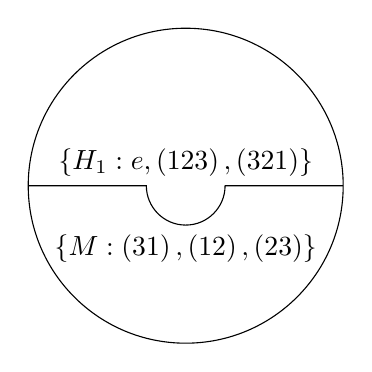
\begin{tikzpicture}
    \draw (0,0) circle [radius=2];
    \draw (2,0) -- (0.5,0) arc [radius=0.5, start angle = 0, end angle = -180] -- (-2,0);
    \node [above] at (0,0) {$\{H_{1}: e, \left(123\right),\left(321\right)\}$};
    \node [below] at (0,-0.5) {$\{M: \left(31\right), \left(12\right), \left(23\right)\}$};
  \end{tikzpicture}
  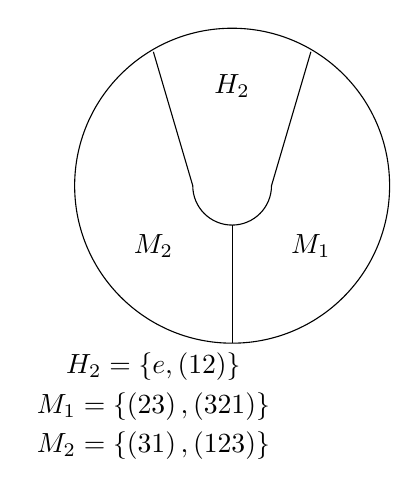
\begin{tikzpicture}
    \draw (0,0) circle [radius=2];
    \draw (1,1.7) -- (0.5,0) arc [radius=0.5, start angle = 0, end angle = -180] -- (-1,1.7);
    \draw (0,-2) -- (0,-0.5);
    \node [above] at (0,1) {$H_{2}$};
    \node [below] at (-1,-0.5) {$M_{2}$};
    \node [below] at (1,-0.5) {$M_{1}$};
    \node [below] at (-1,-2) {$H_{2}= \{e, \left(12\right)\}$};
    \node [below] at (-1,-2.5) {$M_{1}=\{\left(23\right), \left(321\right)\}$};
    \node [below] at (-1,-3) {$M_{2}=\{\left(31\right), \left(123\right)\}$};
  \end{tikzpicture}
  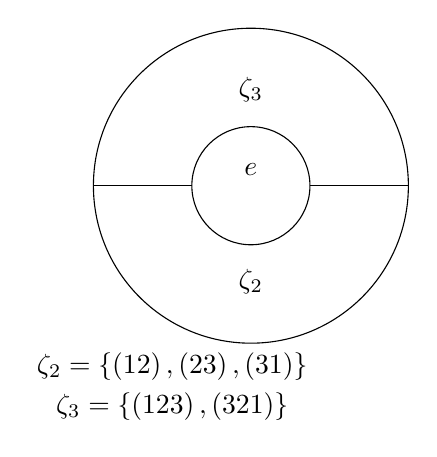
\begin{tikzpicture}
    \draw (0,0) circle [radius=2];
    \draw (0,0) circle [radius=0.75];
    \draw (0.75,0) -- (2,0);
    \draw (-2,0.0) -- (-0.75, 0.0);
    \node [above] at (0,0) {$e$};
    \node [below] at (0,1.5) {$\zeta_{3}$};
    \node [above] at (0,-1.5) {$\zeta_{2}$};
    \node [below] at (-1,-2) {$\zeta_{2}=\{\left(12\right), \left(23\right), \left(31\right)\}$};
    \node [below] at (-1,-2.5) {$\zeta_{3} = \{\left(123\right), \left(321\right)\}$};
  \end{tikzpicture}
  \caption{(a) left cosets of $H_1$ (b) left cosets of $H_2$ (c) classes of $S_3$.}
  \label{fig:1-3}
\end{marginfigure}

The cosets of invariant subgrous are particularly simple and useful.
First, if $H$ is an invariant subgroup, its left cosets are also right cosets\footnote{If $H$ is invariant subgroup $p H p^{-1} = H$, this implies $pH = Hp$.}.
The partitioning of the elements of the full group $G$ into cosets is unique, and a ``factorization'' of $G$ based on this partioning becomes natural.
Let us consider the cosets of an invariant subgroup $H$ as elements of a new group.
The multiplication of two cosets $pH$ and $qH$ is defined as the coset consisting of all products $ph_{i}qh_{j} = \left(pq\right)h_{k}$, where $h_{k} = \left(q^{-1} h_{i} q \right) h_{j} \in H$ provided $h_{i},h_{j} \in H$ and $p,q \in G$.
Since $pH \cdot qH = \left(pq\right) H$, it becomes obvious that (i) $H=eH$ plays the role of the iendtity element; (ii) $p^{-1}H$ is the inverse of $pH$; and (iii) $pH \left(qH \cdot rH \right) = \left(p H \cdot qH \right) \cdot rH = \left(pqr\right) H$.

\textbf{Theorem 1.4} If $H$ is an invarian subgroup of $G$, the set of cosets endowed with the law of multiplication $pH \cdot qH = \left(pq\right)H$ form a group, called the \textit{factor or quotient} group of $G$.
The factor group is denote by $G/H$, it is of order $n_{G}/n_{H}$.

\textrm{Exampel 1}: Consider the inveriant subgroup $H= \{e, a^{2}\}$ of the cyclic group $C_{4}$.
$H$ and coset $M=\{a, a^{3}\}$ form the factor group $C_{4}/H$.
Applying the rule of multiplication of cosets described above, it is straight forward to verify that $HM = M = MH$, $HH = H$, and $MM = H$.
We see that both the subgroup $H$ and the factor group $C_{4}/H$ are of order $2$ and are isomorphic to $C_{2}$.

\textrm{Example 2}: In the case of the permutation group $S_{3}$, $H=\{e, \left(123\right), \left(321\right)\}$ represents an invariant subgroup in Fig.~\ref{fig:1-3} and Tab.~\ref{tab:1-4}.
$G/H$ consists of two elements: $H$ and $M=\{\left(12\right), \left(23\right), \left(31\right)\}$.
We have: $HM= H\cdot \left(ij\right)H= \left(ij\right) H = M = MH$, and $HH= MM = H$.
Therefor, $G/H$ is also isomorphic to the cyclic group of order $2$, $C_{2}$.

\textrm{Example 3}: Consider the discrete translation group $T^{d}=\equiv \Gamma$ and one of its invariant subgroups $\Gamma_{m}$.
The cosets are $\Gamma_{m}$, $T\left(1\right) \Gamma_{m}$, $T\left(2\right) \Gamma_{m}$, \ldots, $T\left(m-1\right) \Gamma_{m}$ and $T\left(m\right) \Gamma_{m} = \Gamma_{m}$.
Hence the factor group $\Gamma/\Gamma_{m}$ is isomorphic to the cyclic group $C_{m}$.
Infinite groups, such as this one, do not behave exactly like finite ones.
For instance, $\Gamma$  and $\Gamma_{m}$ are, in fact, isomorphic to each other even though $\Gamma/\Gamma_{m}$ is non-trival.

\textrm{Example 4}: We state without proof that the translations in $3-$dimensional space form a invariant subgroup of the Euclidean group $E_{3}$; and the factor group is isomrophic to the group of rotations.
This fact forms the basis of important techniques to analyze the Euclidean group and its generalization to $4-$dimensional spacetime---the Poincar\'{e} group.

\section{Homorphisms}
\textbf{Definition 1.11} (homomorphism): A \textit{homomorphism} from a group $G$ to another group $G'$ is a mapping (not necessarily one-to-one) which preserves group multiplication.
In other words, if $g_{i} \in G \to g_{i} \to g_{i}' \in G'$ and $g_{1}g_{2}=g_{3}$, then $g_{1}'g_{2}'=g_{3}'$.

Clearly, isomorphism is a special case of homomorphism.
\begin{figure}
  \centering
    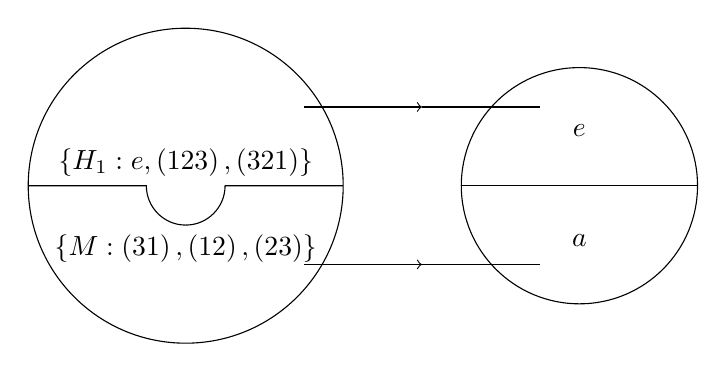
\begin{tikzpicture}
    \draw (0,0) circle [radius=2];
    \draw (2,0) -- (0.5,0) arc [radius=0.5, start angle = 0, end angle = -180] -- (-2,0);
    \node [above] at (0,0) {$\{H_{1}: e, \left(123\right),\left(321\right)\}$};
    \node [below] at (0,-0.5) {$\{M: \left(31\right), \left(12\right), \left(23\right)\}$};
    \draw (5,0) circle [radius=1.5];
    \draw [->] (1.5,1) -- (3,1);
    \draw (3,1) -- (4.5,1);
    \draw [->] (1.5,-1) -- (3,-1);
    \draw (3,-1) -- (4.5,-1);
    \draw (3.5, 0) -- (6.5, 0);
    \node [above] at (5,0.5) {$e$};
    \node [below] at (5,-0.5) {$a$};
  \end{tikzpicture}
  \caption{Homomorphism from $S_3$ to $C_2$.}
  \label{fig:1-4}
\end{figure}

\textrm{Example}:  The mapping from $S_{3}$ to $C_{2}$ depicted in Fig.~\ref{fig:1-4} is a homomorphism.
This follows from the fact that the product of any two element s from $H$ or from $M$ results in an element in H, whereas the product of one element from $H$ with on element from $M$ results in an element in $M$.
This example illustrates the general result that if $G$ has an invariant subgroup $H$, then there exists a natural homomorphism from $G$ to the factor group $G/H: g\in G \to gH \in G/H$.
Group multiplication is preserved b definition.
This result can be turned around to ield the following interesting theorem.

\textbf{Theorem 1.5}: Let $f$ be a homomorphism form $G$ to $G'$.
Denote by $K$ the set of all elements of $G$ whare are mapped to the identity element of $G'$, i.e. $K= \{a \in G; f(a) = e' \in G'\}$.
Then $K$ forms an invariant subgroup of $G$.
Furthermore, the factor group $G/K$ is isomorphic to $G'$.

\section{Direct Products}
Many physically useful symmetry groups are direct products of simpler groups.
When this is the case, it suffices to know the structure and the representations of the smaller groups.

\textbf{Definition 1.12} (Direct Product Group): Let $H_{1}$ and $H_{2}$ be subgroups of a group $G$ with the following properties: (i) every element of $H_{1}$ commutes with any element of $H_{2}$, i.e. $h_{1}h_{2} = h_{2} h_{1}$ for $\forall h_{1} \in H_{1}$ and $\forall h_{2}\in H_{2}$; and (ii) every element $g$ for $G$ can be written uniquely as $g=h_{1}h_{2}$ where $h_{1}\in H_{1}$ and $h_{2}\in H_{2}$.
In this case, $G$ is said to be the direct product of $H_{1}$ and $H_{2}$; symbolically, $G= H_{1}\otimes H_{2}$.

\textrm{Example 1}: Consider the group $C_{6}$ with elements $\{e = a^{6}, a, a^{2}, a^{3}, a^{4}, a^{5}\}$, and the subgroups $H_{1} = \{e, a^{3}\}$ and $H_{2} = \{e, a^{2}, a^{4}\}$.
Cirterion (i)is trivally satisfied because the group is abelian, and (ii) can be verified by $e=ee$, $a = a^{3} a^{4}$ and so on.
Since $H_{1}$ and $H_{2}$ are isomorpism to $C_{2}$ and $C_{3}$, i.e. $H_{1} \simeq C_{2}$ and $H_{2} \simeq C_{3}$, we have $C_{6} \simeq C_{2} \otimes C_{3}$.

If $G= H_{1}\otimes H_{2}$, then both $H_{1}$ and $H_{2}$ must be invariant subgroups of $G$.
\footnote{If $g=h_{1}h_{2}\in G$, and $h_{1}, a \in H_{1}$, $h_{2}\in H_{2}$. Then $g a g^{-1} = h_{1}h_{2} a h_{2}^{-1} h_{1}^{-1} = h_{1} a h_{1}^{-1} \in H_{1}$ for all $g$ and $a$.}
Now, we can form the quotient group $G/H_{2}$ and prove that, $G/H_{2} \simeq H_{1}$.
However, the converse to the above is not true!
Let $H$ be an invariant subgroup of $G$ and $H'= G/H$.
It does not follow that $G = H \otimes H'$.


%%% Local Variables:
%%% mode: latex
%%% TeX-master: "main"
%%% End:

\chapter{GROUP REPRESENTATIONS}

\section{Representations}
\textbf{Definition 2.1} (Representations of a Group): If there is a homomorphism from a group $G$ to a group operatures $U\left(G\right)$ on a linear vector space $V$, we say that $U\left(G\right)$ forms a \textit{representation} of the group $G$.
The \textit{dimension of the representations} is the dimension of the vector space $V$.
A representation is said to be \textit{faithful} if the homomorphism is alo an isomorphism.
A \textit{degenerate representation} is one which is not faithful.

To be more specific: the representation is a mapping
\begin{equation*}
  g \in G \xRightarrow[above]{U} \left(g\right)
\end{equation*}
where $U\left(g\right)$ is an operator on $V$, such that
\begin{equation}
  \label{eq:2.1-1}
  U\left(g_{1}\right) U\left(g_{2}\right) = U \left(g_{1} g_{2}\right)
\end{equation}
i.e., the representation operators satisfy the same rules of multiplication as the original group elements.

Consider the case of a finite-dimensional representation.
Choose a set of basis vectors on $V$.
The operators $U\left(g\right)$ are then realized as $n\times n$ matrices $D\left(g\right)$ as follows\footnote{where $j$ is the row index and $i$ is the column index}:
\begin{equation}
  \label{eq:2.1-2}
 U\left(g\right) \ket{e_{i}} = \ket{e_{j}} D\left(g\right)^{j}_{i}, ~ ~ ~ g \in G.
\end{equation}
And from Eq.~\eqref{eq:2.1-1}, we have
\begin{equation}
  \label{eq:2.1-3}
 D\left(g_{1}\right) D\left(g_{2}\right) = D\left(g_{1}g_{2}\right)
\end{equation}
And since $D\left(G\right)$ satisfy the same algebra as $U\left(G\right)$, the group of matrices $D\left(G\right)$ forms a \textit{matrix representation} of $G$.

\textrm{Example 1}: The trivial $1-$dimenional representation for every group $G$.
Let $V=C$, and $U\left(g\right) = 1$ for all $g \in G$.
Then $g\in G \longrightarrow 1$ forms a representation.

\textrm{Example 2}: Let $G$ be a group of matrices, $V=C$, and $U\left(g\right) =\det g$.
This define non-trivial one-dimenional representation since $\det g_{1} \det g_{2} = \det g_{1}g_{2}$.

\textrm{Example 4}: Let $G$ be the dihedral group $D_{2}$ consisting of $e$ (identity), $h$ (reflection about the $Y-$axis), $v$ (reflection about the $X-$axis), and $r$ (rotation by $\pi$ around the origin) as described at Tab.~\ref{tab:1-3} and Fig.~\ref{fig:1-1}.
Let $V_{2}$ be the two-dimensional Euclidean space with basis vector $\left(\hat{e}_{1}, \hat{e}_{2}\right)$.
By referring to Fig.~\ref{fig:2-1} and making use of the definition Eq.~\eqref{eq:2.1-2}, we easily infer
\begin{equation}
  \label{eq:2.1-4}
  D\left(e\right) =
  \begin{bmatrix}
    1 & 0 \\
    0 & 1
  \end{bmatrix}
  D\left(h\right) =
  \begin{bmatrix}
    -1 & 0 \\
    0 & 1
  \end{bmatrix}
  D\left(v\right) =
  \begin{bmatrix}
    1 & 0 \\
    0 & -1
  \end{bmatrix}
  D\left(r\right) =
  \begin{bmatrix}
    -1 & 0 \\
    0 & -1
  \end{bmatrix}
\end{equation}
It is straightforward to very that the mapping $g\longrightarrow D\left(g\right)$ is a homomorphism, hence these matrices form a $2-$dimensional representation of the $D_{2}$ group.
\begin{figure}
  \centering
  \begin{tikzpicture}
    \draw [<->] (-2,0) -- (2,0);
    \draw [<->] (0,-2) -- (0,2);
    \draw [dashed] (0,0) circle [radius=2];
    \node [right] at (2,0) {$\hat{e}_{1}, ~ v\hat{e}_{1}$};
    \node [above] at (0,2) {$\hat{e}_{2}, ~ h\hat{e}_{2}$};
    \node [left] at (-2,0) {$r\hat{e}_{1}, ~ h\hat{e}_{1}$};
    \node [below] at (0,-2) {$v\hat{e}_{2}, ~ r\hat{e}_{2}$};
  \end{tikzpicture}
  \caption{$D_2$ transformations}
  \label{fig:2-1}
\end{figure}

\textrm{Example 5}: Let $G$ be the group of continuous rotations in a plane around origin $O$, $G=\{R\left(\phi\right), 0\leq \phi \leq 2\pi\}$.
Let $V_{2}$ be the two-dimensional Euclidean space, since
\begin{align}
  \label{eq:2.1-5}
  \hat{e}_{1}' &= \hat{e}_{1} \cos \phi + \hat{e}_{2} \sin \phi \\
  \hat{e}_{2}' &= -\hat{e}_{1} \sin \phi + \hat{e}_{2} \cos \phi \nonumber
\end{align}
we have
\begin{equation}
  \label{eq:2.1-6}
  D\left(\phi\right) =
  \begin{bmatrix}
    D_{1}^{1}=\cos \phi & D_{1}^{2}=-\sin \phi \\
    D_{2}^{1}=\sin \phi & D_{2}^{2}=\cos \phi
  \end{bmatrix}
\end{equation}
Since according Eq.~\eqref{eq:2.1-2}, $U \ket{e_{1}} = \ket{e_{1}} D\left(\phi\right)_{1}^{1}+ \ket{e_{2}} D\left(\phi\right)_{1}^{2}$.
However, if $\mathbf{x}$ is an arbitrary vector in $V_{2}$, $\mathbf{x} = \hat{e}_{j} x^{j}$, then
\begin{align}
  \label{eq:2.1-7}
  \mathbf{y} &= U\left(\phi\right) \mathbf{x} = \hat{e}_{j} y^{j} \\ \nonumber
  y^{j} &= D\left(\phi\right)^{j}_{i} x^{i} \\ \nonumber
  \begin{bmatrix}
    y^{1} \\
    y^{2}
  \end{bmatrix}
  &=
  \begin{bmatrix}
  \cos \phi & -\sin \phi \\
  \sin \phi & \cos \phi
  \end{bmatrix}
  \begin{bmatrix}
  x^{1}\\
  x^{2}
  \end{bmatrix}
\end{align}

As we can see, different groups may be realized on the same vector space.
Here, the $2-$dimensional Euclidean space $V_{2}$ is seen to provide representations for the two finite groups $D_{2}$, $D_{3}$ as well as the continuous group $R\left(2\right)$

\textrm{Example 7}: Let $V_{f}$ be te space of complex-valued linear homogeneous founctions $f$ of two real varibales $\left(x,y\right)$:
\begin{equation}
  \label{eq:2.1-8}
  f\left(x,y\right) = a x + by
\end{equation}
where $\left(a,b\right)$ are arbitary complex coefficients.
Interpret $\left(x,y\right)$ as the components of a vector $\mathbf{x}$ in a $2$-dimenional Euclidean space $V_{2}$.
Then the group operations from previos examples will induce the following transformation in the function space $V_{f}$
\begin{equation}
\label{eq:2.1-9}
f \xRightarrow{g \in G} f'\left(x^{1},x^{2}\right) \equiv f \left(x'^{1},x'^{2}\right)
\end{equation}
where $\mathbf{x}' = U\left(g^{-1}\right) \mathbf{x}$.
It is straightforward to show that the mapping defined by Eq.~\eqref{eq:2.1-9} is a homomorphism; for if $g" g' = g$ then
\begin{align}
\label{eq:2.1-10}
f \xRightarrow{g'} f' ~ ~ ~ f' \left(\mathbf{x}\right) &= f \left[ U\left(g'\right)^{-1} \mathbf{x} \right] \\ \nonumber
f' \xRightarrow{g"} f" ~ ~ ~ f"\left( \mathbf{x} \right) &= f' \left[ U\left(g"\right)^{-1} \right] = f \left[U\left(g'\right)^{-1} U\left(g"\right)^{-1} \mathbf{x} \right] \\ \nonumber
  &= f\left[U\left(g"g'\right)^{-1} \mathbf{x}\right] = f\left[ U\left(g\right)^{-1} \mathbf{x}\right]
\end{align}
Therefore, the set of transformation defined by Eq.~\eqref{eq:2.1-9} forms a representation of the group $G$.

\textbf{Theorem 2.1:} (i) If the group $G$ has a non-trivial invariant subgroup $H$, then any representation of the factor group $K=G/H$ is also a representaion of $G$.
This representaion must be degenerate; (ii) Conversely, if $U \left( G \right)$ is a degenerate representation of $G$, then $G$ has at least one invariant subgroup $H$ such that $U \left( G \right)$ defines a faithful representation of the factor group $G/H$.

A immediate corollay of this theorem is that all representations of simple groups are faithful.

\section{Irreducible, Inequivalent Representations}
The first type of redundacy is due to similarity transformation.

\textbf{Definition 2.2} (Equivalence of Representations): Two representations of a group $G$ related by a similarity transfromation are said to be equivalent.

By seeking characterizations of the representation which are invariant under similarity transfomations, we can tell the two representations are equivalant or not.
The trace $\tr A$ and determinant $\det A$ are two characterizations which are independent of the choice of the base.

\textbf{Definition 2.3} (Characters of a Representation): The \textit{character} $\chi \left( g \right)$ of $g \in G$ in a represenation $U \left( G \right)$ is defined to be $\chi \left( g \right) = \Tr U \left( g \right)$.
All group elements in a given class of $G$ have the same characters, becase $\Tr D \left( p \right) D \left( g \right) D \left( p^{-1} \right)= \Tr D \left( g \right)$.
Therefor, the group character is a function of the class-label only.

A second type of redundacy concerns direct sum representations.

\textbf{Definition 2.4} (Invariant Subspace): Let $U \left( G \right)$ be a representation of $G$ on the vector space $V$, and $V_{1}$ be a subspace of $V$ with the property that $U \left( g \right) \ket{x} \in V_{1}$ for all $\mathbf{x} \in V_{1}$ and $g \in G$.
$V_{1}$ is siad to be an \textit{invariant subspace} of $V$ with repsect ot $U \left( G \right)$.
An invariant subspace is \textit{mimimal} or \textit{proper} if it does not contain any non-trival invariant subspace with respect ot $U \left( G \right)$.

Examples of trivial invariant subspaces of $V$ with respect to $U \left( G \right)$ are: (i) the space $V$ itself, and (ii) the subspace consisting only of the null vector.

\textbf{Definition 2.5} (Irreducibel Representations): A representation $U \left( G \right)$ on $V$ is \textit{irreducible} if there is no non-trivial invariant subspace in $V$ with respect to $U \left( G \right)$.
Otherwise, the representation is \textit{reducible}.
In latter case, if the orthogonal complement\footnote{If $V_{1}$ is a subspace of $V$, the orthogonal complement of $V_{1}$ consists of all vectors in $V$ which are orthogonal to very vector in $V_{1}$. For finite-dimensional vector spaces, at least, the orthogonal complement of $V_{1}$ also forms a subspace, called $V_{2}$, then we have $V = V_1 \oplus V_2$.}of the invariant subspace is also invariant with respect to $U \left( G \right)$, then the represenation is said to be \textit{fully reducible or decomposable.}

\textrm{Example 1}: Consider the action of the dihedral group $D_2$ on the $2-$dimensional Euclidean space $V_2$ as described in Fig.~\ref{fig:2-1} and Eq.~\eqref{eq:2.1-4}.
The $1-$dimensional subspace spanned by $\hat{e}_1$ is invariant under all four group operations, $D_2 \left( g \right) \hat{e}_1 = \pm \hat{e}_1$.
The same is true for the subspace spaned by $\hat{e}_2$.
Thus the $2-$dimensional representation of the group given by Eq.~\eqref{eq:2.1-4} is therefore a reducible representation.

\textrm{Example 2}: The $1-$dimensional subspace spanned by $\hat{e}_{1}$ or $\hat{e}_2$ is not invariant under the group $\mathbf{R} \left( 2 \right)$.
However, if we form the following linear combinations of vectors,
\begin{equation}
  \label{eq:2.2-1}
 \hat{e}_{\pm} = \frac{1}{\sqrt{2}} \left( \mp \hat{e}_1 - i \hat{e}_2 \right)
\end{equation}
it is straightforward to show that:
\begin{align}
  \label{eq:2.2-2}
  U \left( \phi \right) \hat{e}_+ &= \hat{e}_+ e^{-i\phi} \\ \nonumber
  U \left( \phi \right) \hat{e}_- &= \hat{e}_- e^{i\phi}
\end{align}
Therefore, the $1-$dimensional spaces spanned by $\hat{e}_{\pm}$ are individually invariant under the rotation group $R \left( 2 \right)$.
The $2-$dimensional representation given by Eq.~\eqref{eq:2.1-6} can be simplified if we make a change of basis to the eigenvectors $\hat{e}_{\pm}$.
In this new basis,
\begin{equation}
  \label{eq:2.2-3}
  D' \left( \phi \right) =
  \begin{bmatrix}
    e^{-i\phi} & 0 \\
    0 & e^{i\phi}
  \end{bmatrix}
\end{equation}
The new matrices can be obtained form the old one in Eq.~\eqref{eq:2.1-6} by a similarity transformation which is defined by Eq.~\eqref{eq:2.2-1}.

Let us look at the general matrix form of a reducible representation.
If $V_1$ is an $n_1-$dimensional invariant subspace with respect to $U \left( G \right)$, we can always choose a set of basis vectors in $V$ such that the first $n_1$ vectors are in $V_1$.
Since, for all $g\in G$
\begin{equation}
 U \left( g \right) \ket{e_i} = \ket{e_j} D \left( g \right)^j_i \in V_1 ~ ~ ~ \text{for}~ i= 1, \dots, n_{1} \nonumber
\end{equation}
we conclude that $D \left( g \right)_i^j = 0$ for $i=1, \dots, n_1$ and $j= n_1+1, \dots, n$.
Therefor, the matrix representation is of the form
\begin{equation}
  \label{eq:2.2-4}
  D \left( g \right) =
  \begin{bmatrix}
    D_1 \left( g \right) & D' \left( g \right) \\
    0 & D_2 \left( g \right)
  \end{bmatrix}
\end{equation}
If $D \left( g \right)$ and $D \left( g' \right)$ are both of this form, then the product $D \left( gg' \right)$ is also of this form, and that $D_i \left( gg' \right) = D_i \left( g \right) D_i \left( g' \right)$ for $i=1,2$.
Thus, all esential properties of $D \left( G \right)$ are already contained in the representations $D_i \left( G \right)$.

We see that if $U \left( G \right)$ is a representation of the group $G$ on $V$ and $V^{\mu}$ is an invariant subspace of $V$ respect to $G$, then by restricing the action of $U \left( G \right)$ to $V^{\mu}$, we obtain a lower-dimension representation $U^{\mu} \left( G \right)$.
If the subspace $V^{\mu}$ cannot be further reduced, $U^{\mu} \left( G \right)$ is an irreducible represenation, and we say that $V^{\mu}$ is a \textrm{proper or irreducible invariant subspace} with respect to $G$.

\section{Unitary Representations}
\textbf{Definition 2.6} (Unitary Representation): If the group representation space is a inner product space, and if the operators $U \left( g \right)$ are unitary for $g \in G$, then the representation $U \left( G \right)$ is said to be a \textit{unitary representation}.

Because symmetry transformation are naturally associated with unitary operators, unitary representations play a cnetral role in studying symmetry groups.

\textbf{Theorem 2.2:} If a unitary representation is reducible, then it is alos decomposable i.e., fully reducible.

\textbf{Theorem 2.3:} Every representation $D \left( G \right)$ of a finite group on an inner product space is equivalent to a unitary representation, i.e., there exist a similar transformation such that $S D \left( g \right) S^{-1}$ is unitary.






%%% Local Variables:
%%% mode: latex
%%% TeX-master: "main"
%%% End:


\bibliography{mybib}{}
\bibliographystyle{abbrv}
\end{document}

%%% Local Variables:
%%% mode: latex
%%% TeX-master: t
%%% End:
